\documentclass{article}
\usepackage{graphicx}
\usepackage[margin=1.5cm]{geometry}
\usepackage{amsmath}

\begin{document}

\title{Thursday Reading Assessment: Unit 3, Magnetic Forces and Fields}
\author{Prof. Jordan C. Hanson}

\maketitle

\section{Memory Bank}

\begin{itemize}
\item $V_{\rm H} = B l v$ ... The Hall voltage, given external B-field, height of conductor, $l$, and the drift velocity $v$.
\item $V_{\rm H} = (I B l)/(n q A)$ ... The Hall voltage, given external B-field, height of the conductor, $l$, the number density, $n$, the charge per carrier, $q$, and the conductor area $A$.
\item $\vec{F} = I\vec{L} \times \vec{B}$ ... The Lorentz force on a current.
\end{itemize}

\section{The Hall Effect}

\begin{figure}[ht]
\centering
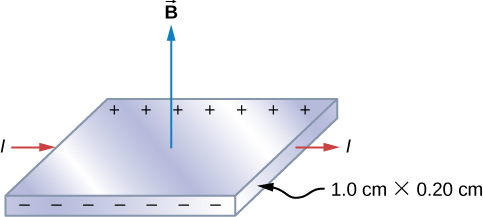
\includegraphics[width=0.35\textwidth]{hall.jpeg}
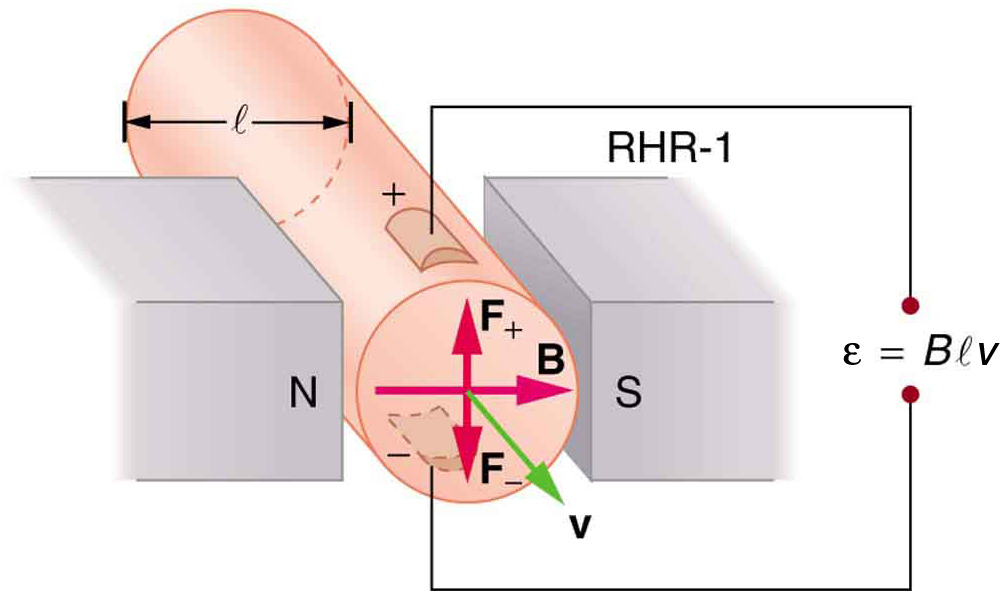
\includegraphics[width=0.25\textwidth]{hall2.jpeg} \hspace{0.2cm}
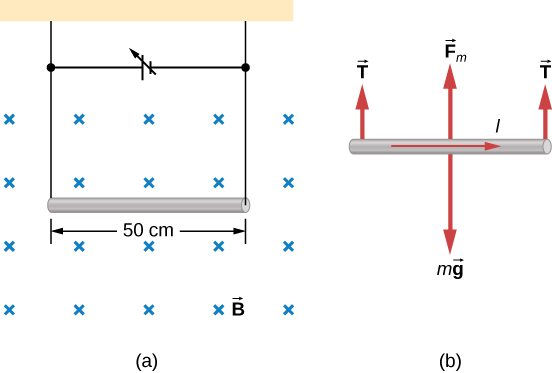
\includegraphics[width=0.3\textwidth]{forceWire.jpeg}
\caption{\label{fig:hall} (Left) A geometry in which the Hall effect occurs. (Middle) A Hall-probe is used to measure fluid flow. (Right) A force is placed on a wire in a B-field.}
\end{figure}

\begin{enumerate}
\item Figure \ref{fig:hall} (left) shows a silver ribbon whose cross section is 1.0 cm by 0.20 cm. The ribbon carries a current of 100 A from left to right, and it lies in a uniform magnetic field of magnitude 1.5 T. Using a density value of $n = 6 \times 10^{28}$ electrons per cubic meter for silver, find the Hall potential between the edges of the ribbon. \\ \vspace{2cm}
\item A Hall probe is used to measure fluid flow (Fig. \ref{fig:hall}, middle).  Suppose a small tube carries fluid moving at velocity $v$, in a 0.8 T B-field, and the tube is 1 cm wide.  The Hall voltage is $0.5 \times 10^{-6}$ Volts.  What is $v$? \\ \vspace{1cm}
\end{enumerate}

\section{Magnetic Forces on a Wire}

\begin{enumerate}
\item Consider Fig. \ref{fig:hall}, right, in which a 0.5 T B-field suspends a 10 gram wire of length 0.5 meters.  What is the current in the wire, and in which direction?
\end{enumerate}

\end{document}
